 %\pdfoutput=1
\documentclass[conference]{IEEEtran}
\IEEEoverridecommandlockouts
% The preceding line is only needed to identify funding in the first footnote. If that is unneeded, please comment it out.
\usepackage[T1]{fontenc}
\usepackage{cite}
\usepackage{mathtools}
\usepackage{stackengine}
\def\delequal{\mathrel{\ensurestackMath{\stackon[1pt]{=}{\scriptstyle\Delta}}}}
\usepackage{amsmath,amssymb,amsfonts}
\usepackage{amsmath,epsfig,cite,amsfonts,amssymb,psfrag,subfig}
\usepackage{graphicx}
\usepackage{textcomp}
\usepackage{xcolor}
\usepackage{algorithm}
\usepackage[noend]{algpseudocode}
\usepackage{amsthm}
\def\BibTeX{{\rm B\kern-.05em{\sc i\kern-.025em b}\kern-.08em
    T\kern-.1667em\lower.7ex\hbox{E}\kern-.125emX}}
\allowdisplaybreaks
\newtheorem{remark}{Remark}
\newtheorem{theorem}{Theorem}
\newtheorem{lemma}{Lemma}
\newtheorem{proposition}{Proposition}
\newtheorem{corollary}{Corollary}
\newcommand{\diag}{\mathop{\mathrm{diag}}}
\DeclareMathOperator{\E}{\mathbb{E}}
\usepackage[margin=0.7in]{geometry}
\setlength{\columnsep}{11mm}
\begin{document}

\title{Dynamic RB scheduling for different slices of eMBB and URLLC in the O-RAN system \vspace{-.1cm}
}
%
%\author{\IEEEauthorblockN{1\textsuperscript{st} Mojdeh Karbalaee Motalleb}
%\IEEEauthorblockA{\textit{Electrical and Computer Engineering} \\
%\textit{Tehran University}\\
%Tehran, Iran \\
%mojdeh.karbalaee@ut.ac.ir}
%\and
%\IEEEauthorblockN{2\textsuperscript{nd} Vahid Shah-Mansouri}
%\IEEEauthorblockA{\textit{Electrical and Computer Engineering} \\
%\textit{Tehran University}\\
%Tehran, Iran \\
%vmansouri@ut.ac.ir}
%\and
%\IEEEauthorblockN{3\textsuperscript{rd} Salar Nouri Naghadeh}
%\IEEEauthorblockA{\textit{Electrical and Computer Engineering} \\
%\textit{Tehran University}\\
%Tehran, Iran \\
%salar.nouri@ut.ac.ir}
%}
%%%%%  \author{
%%%%%    \IEEEauthorblockN{Mojdeh Karbalaee Motalleb}
%%%%%    \IEEEauthorblockA{School of ECE, College of Engineering, University of Tehran, Iran \\
%%%%%    Email: \{mojdeh.karbalaee\}@ut.ac.ir,
%%%%%    \vspace{-.2cm}
%%%%%  }
%%%%%  }

\maketitle

\begin{abstract}

\end{abstract}
\section{Introduction} 

%\begin{figure*}
%  \centering 
%    \includegraphics[scale = 0.5]{finalDraw1.pdf}
%    %\includegraphics[max height=30cm,max width=9.5cm]{Drawing15.eps}
%    %\includegraphics[width=\textwidth]{finalDraw.pdf}
%  \caption{Network sliced ORAN system}
%  \label{fig:1}
%\end{figure*}

\section{System Model and Problem Formulation}
\subsection{System Model}
Consider two different services of eMBB and URLLC in O-RAN architecture; each offers various applications.
Therefore, we assume two different slices for eMBB and URLLC services. The system is serving a set of $\mathcal{U}_e$ eMBB single-antenna user equipment(UE) and a set of $\mathcal{U}_u$ URLLC UE. Suppose we have $K$ preallocated resource blocks (RBs) for serving these two services.
 Moreover, the system considers having  virtual network function (VNFs) in O-DU and O-CU to process packets. Each service has its VNFs for processing due to the isolation of slices.
Let the system have $M_s^{d}$ VNFs for the processing of O-DU, $M_s^{c}$ VNFs for the processing of O-CU-UP of eMBB and URLLC services ($ s \in \{e, u\}$ for eMBB and URLLC respectively).
A VNF is a system's core component. Every VNF instance is hosted on a virtual machine (VM) using resources from the data centers. 
Moreover, we assume there is a cell with one O-RU that serves UEs.
Furthermore, we suppose the channel distribution is known.
The eMBB services generally use more than a one-time slot. But URLLC services use part of a time slot (mini-slot) since it has a short packet transmission. 
By using the PF principle, we currently allocate RBs at the beginning of each eMBB time slot, a scheduling strategy that balances throughput and fairness \cite{shi2022risk}. 
However, puncturing the URLLC once requested service is necessary as it requires very low latency.
\subsection{The Achievable Rate}
%\begin{figure}
%  \centering 
%    \includegraphics[scale = 0.4]{EU.pdf}
%    %\includegraphics[max height=30cm,max width=9.5cm]{Drawing15.eps}
%    %\includegraphics[width=\textwidth]{finalDraw.pdf}
%  \caption{RB scheduling}
%  \label{fig:2}
%\end{figure}

The achievable data rate and the expectation of the achivable data rate for the $i^{th}$ UE request eMBB slice can be written as $\mathcal{R}_{i}^{e}(t)$, and $\bar{\mathcal{R}}_{i}^e(t)$, respectively.
\begin{equation}\label{eq1}
\begin{split}
\mathcal{R}_{i}^e(t) &= \sum_{k = 1}^K e^k_i(t) B (1-{n^k_i(t)}) \log_2({1+\frac{p^k_i(t)h^k_i(t)}{B \times N_0}}),\\
\bar{\mathcal{R}}_{i}^e(t) &= \E_{h}[\mathcal{R}_{i}^e(t)],
\end{split}
\end{equation}
where $B$ is the bandwidth of RBs. Also, $B\times N_0$ denotes the power of Gaussian additive noise. 
Moreover, $e^k_i(t)\in \{0,1\}$ is a binary variable that illustrates whether RB $k$ is assigned to the $i^{th}$ eMBB UE or not. 
$p^k_i(t)$ represents the transmission power allocated by O-RU to $i^{th}$ UE of eMBB using PRB $k$.
$h^k_i(t)$ is the channel gain of a wireless link from 
O-RU to the $i^{th}$ eMBB UE using $k^{th}$ PRB which is Rayleigh fading.
Furthermore, $n^k_i(t)$ denotes the percentage of RB $k$ using eMBB $i$ that is punctured by the set of URLLC service is indicates as follows,
%\begin{equation}
%n^k_i(t) = \psi^k_i(t) \frac{\sum_{j \in \mathcal{U}_2}{\zeta}^u_{j}(t){\nu}^u \tau}{S_{max}(t)\tau},
%\end{equation}
%Where, $\psi^k_i(t)$ is the probability of puncturing eMBB UE $i$ using RB $k$.
%Furthermore, ${\zeta}^u(t)$ is the arrival rate of URLLC UEs (arrival/slot/user).
%Moreover, $\mathcal{U}_2$ is the set of URLLC UEs in the system.
%In addition, $\nu^u$ is the URLLC packet size, and $\tau$ is the number of slot per second (slot/sec).
%Assume the packet arrival of URLLC UEs follows a Poisson process with arrival rate $\lambda(t)$.
%Therefore, the arrival data rate of URLLC $j$ is $\lambda_j(t) = {\zeta}^u_{j}(t){\nu}^u \tau$ .
%Moreover, $S_{max}(t)$ is the flow density refers to how much data the system can handle for all URLLC users at any given time (bits/slot).
\begin{equation}
n^k_i(t) = \frac{x^k_i(t)}{L}
\end{equation}
where, $x^k_i(t)$ is the number of punctured mini-slot of RB k that is used by eMBB UE i. Also, $L$ is the number of mini-slots in each RB \cite{alsenwi2021intelligent}.

Moreover, we have $\sum_i e_i^k(t)\le 1$ to guarantee that each RB is allocated to a maximum of one eMBB UE.

Since the blocklength in URLLC is finite, the achievable data rate for the $j^{th}$ UE request in the URLLC service, is not achieved from Shannon Capacity formula. So, for the short packet transmission the achievable data rate and its expectation is written as follow, respectively, 
\begin{equation}\label{eq11}
\begin{split}
\mathcal{R}_{j}^u(t) &= \sum_{i = 1}^{U_e}\sum_{k=1}^K m_i^{k}(t) B \log_2({1+\frac{p^k_j(t)h^k_j(t)}{B \times N_0}})- \zeta_{j}^k(t),\\
\bar{\mathcal{R}}_{j}^u(t) &= \E_{h}[\mathcal{R}_{j}^u(t)],
\end{split} 
\end{equation}
where $\zeta_{j}^k(t) = \log_2({e})Q^{-1}(\epsilon) \sqrt{\frac{C_{j}^k(t)}{N_{j}^k(t)}})$
where $\epsilon$ is the transmission error probability, $Q^{-1}$ is the inverse of Q function (i.e., Gaussian),
$C_{j}^k(t) = 1 - \frac{1}{(1+\rho_{j}^k(t))^2}$ depicts the channel dispersion of $j^\text{th}$ UE of URLLC service, puncturing mini-slots of RB $k$ and
$N_{j}^k(t)$ represents the blocklength of it. Moreover, $\rho_{j}^k(t)=\frac{p^k_j(t)h^k_j(t)}{B \times N_0}$ is the SNR of UE $j$ in URLLC service. 
Also, $m_i^{k}(t) $ is denoted as follow
\begin{equation}
m_i^{k}(t)= \frac{e_i^k(t)n^k_i(t)}{|\mathcal{U}_u|},
\end{equation}
where, $|\mathcal{U}_u|$ is the number of URLLC UEs in the system.
%The channel gain is assumed to be known with errors, the imperfection of channel estimation is
%modeled as follows
%\begin{equation}
%h^k_j(t) = \hat{h}^k_j(t) + \Delta h^k_j(t)
%\end{equation}
%Where, $\Delta h^k_j(t)$ denotes the estimation error with a Guassian distribution of
% \begin{equation}
%\Delta h^k_j(t)\backsim \mathcal{N}(0,\boldsymbol{\phi^k}^2),
%\end{equation}
\subsection{Mean Delay}
In this section, the mean processing delay for each service is determined.
Let us suppose the mean total processing time is
\begin{subequations} 
\begin{alignat}{4}
T^{\text{tot}} &= T^{RU} + T^{\text{proc}},\\
T^{\text{proc}} &= T^{DU} + T^{CU}.
\end{alignat}
\end{subequations} 
We assume that the packet arrival rate of each UE $\mathfrak{i}$ in each service s follows a Poisson process with arrival rate $\lambda_{\mathfrak{i},s}(t)$.
%Thus, we have $\lambda_j(t) = {\zeta}^u_{j}(t){\nu}^u \tau$.
Therefore, the mean arrival data rate of the O-CU-UP layer is $\alpha^C_{s}(t) = \sum_{\mathfrak{i}\in \mathcal{U}_s}\lambda_{\mathfrak{i},s}(t)$, $s \in \{e,u\}$ which is for eMBB and URLLC service, respectively.
Assume the mean arrival data rate for URLLC slice ($\alpha$) is approximately equal to the mean arrival data rate of the O-DU ($\alpha^D$). so $\alpha_s(t) = \alpha^C_{s}(t) \approx \alpha^D_s(t)$, $s \in \{e,u\}$.
Because the amount of data traffic transferred along the route (regardless of frame changes) is constant.
Since, by using Burke’s theorem, the mean arrival data rate of the second layer, which are processed in the first layer, is still poisson with rate $\alpha$.
It is assumed that there are load balancers in each layer for each service to divide the incoming traffic to VNFs equally. %\cite{frdl,luong2018novel,luong2018novel1}.
Suppose the baseband processing of each VNF is depicted as M/M/1 processing queue.
Each packet is processed by one of the VNFs of a slice. So, the mean delay for the each slice ($s \in \{e,u\}$ which is for eMBB and URLLC service, respectively) in the O-DU,and the O-CU is modeled as M/M/1 queue, is formulated as follows, respectively \cite{SystemCostMinimization,luong2018joint,luong2018novel},
\begin{equation}
\begin{split}
T^{DU}_s &= \frac{1}{\mu^d_s - \alpha_s(t)/{M^{d}_s(t)}},\\
T^{CU}_s &= \frac{1}{\mu^c_s - \alpha_s(t)/{M^{c}_s}(t)},\\
\end{split}
\end{equation}
where $M^{d}_s(t)$,and $M^{c}_s(t)$ are the variables that depict the number of VNFs in O-DU,and O-CU-UP, respectively. 
Moreover, $1/\mu^d_s$, and $1/\mu^c_s$ are the mean service time of the O-DU, and O-CU layers, respectively.
Besides, $\alpha_s$ is the  arrival rate which is divided
by load balancer before arriving to the VNFs. The arrival rate of each VNF in each layer for each slice is $\alpha_s/{M^{l}_s}$ $ l \in \{d,c\}$.

Suppose the mean transmission delay of the $\mathfrak{i}^{th}$ UE of the service s ($s \in \{e,u\}$which is for eMBB and URLLC service, respectively) on the wireless link is denoted by
$T_{\mathfrak{i},s}^{RU}(t)$.
 Assume the arrival data rate of wireless link for each UE $\mathfrak{i}$ of service s is $\lambda_{\mathfrak{i},s}(t)$
As a result, we have $\sum_{\mathfrak{i} \in \mathcal{U}_s} {\mathfrak{i},s}(t) = \alpha_s(t)$, $s \in \{e,u\}$.
Moreover, The service time of transmission queue for UE $\mathfrak{i}$ requesting service s has
an exponential distribution with mean $1/R_{\mathfrak{i}}^s(t)$ and can be modeled as a M/M/1 queue \cite{SystemCostMinimization,luong2018joint,luong2018novel}.
 
Therefore, the mean delay of the transmission layer for UE $\mathfrak{i}$ in slice s is
\begin{equation}
 T_{\mathfrak{i},s}^{RU}(t) = \frac{1}{{\mathcal{R}}_{\mathfrak{i}}^s(t) - \lambda_{\mathfrak{i},s}(t)}.
\end{equation}


\subsection{Reliability of URLLC}
As we know, UEs request URLLC services, require services with low latency.
For the M/M/1 system, the probability of the delay for URLLC service in the O-RU is as follow, 
\begin{equation}
P_r\{T_{j,u}^{RU} \geq T^{RU}_{\text{max}}\} = e^{-({R}_{j}^u - \alpha)T^{RU}_{\text{max}}}
\end{equation} 
Also, we do not consider the reliability for O-CU and O-DU.

\subsection{Problem Statement}
%In this system, the goal is to minimize the cost of the system.
%The total power cost of O-RUs for transmitting data to UE is depicted as follow
%\begin{equation}
%P_{tot} = \sum_{r=1}^{R}P_r
%\end{equation}
In this paper, we strive to maximize the sum rate of all eMBB UEs and minimize the delay of URLLC UEs while imposing constraints on their performance based on their QoS.
The optimization problem is formulated as follow,

\begin{subequations} \label{mainP}
\begin{alignat}{4}
\max\limits_{ \boldsymbol{E}, \boldsymbol{X},\boldsymbol{M}, \boldsymbol{P} } &  \sum_i {\mathcal{R}}_{i}^e(t) - \eta \sum_j T^{\text{tot}, u}(t)       \ \\
\text{subject to} \quad  & {\mathcal{R}}_{i}^e(t) \geq  \mathcal{R}_{min}^e \quad \forall i \in \mathcal{U}_e, \label{p1} \\
& \sum_k^K \sum_i^{U_e} p^k_i(t) \leq P_{\text{max}},  \label{p1-1} \\ 
& Pr\{{\mathcal{R}}_{i}^e(t) \leq {R}_{min}^e\}  \leq \epsilon,\quad \forall i \in \mathcal{U}_e, \label{p2}\\
&T^{\text{tot}, e}_i(t)  \leq T_{min}^e  \quad \forall i \in \mathcal{U}_e, \label{p2-1} \\
&T^{\text{tot}, u}_j(t)  \leq T_{min}^u  \quad \forall j \in \mathcal{U}_u, \label{p3} \\
& {\mathcal{R}}_{j}^u(t) \geq  \mathcal{R}_{min}^u \quad \forall j \in \mathcal{U}_u, \label{p3-1} \\
&Pr\{T^{\text{RU}, u}_j(t) \geq T_{min}^u\} \leq \epsilon  \quad \forall j \in \mathcal{U}_u, \label{p4} \\
&\sum_{i=1}^{U_1}e^k_i(t)\leq 1 \quad \forall k \in \{1,...,K\},\label{p5} \\
&e^k_i(t)\in \{0,1\}  \quad \forall i,k, \label{p6} \\
& x^k_i(t)\in \{0,1,...,L\}  \quad \forall i,k, \label{p7} \\
& \mu^l_s \geq \alpha_s/M^l_s \quad l \in \{c,d\}, s\in\{e,u\}, \label{p8} \\
& {\mathcal{R}_{\mathfrak{i}}}^s(t) \geq {\lambda}_{\mathfrak{i},s}(t) \quad \forall \mathfrak{i} \in \mathcal{U}_s, s\in \{e,u\}\label{p9} \\
& 0 \leq M^l_e  + M^l_u \leq M_{max}^l  \quad l \in \{c,d\},\label{p10}\\
& 0 \leq M^l_e, M^l_u  \quad l \in \{c,d\},\label{p011}
\end{alignat}
\label{constraints}
\end{subequations}
Where, \eqref{p1}, guarantees the minimum data rate of eMBB UEs, also \eqref{p1-1} indicates the power allocation constraints.
\eqref{p2}, supports the reliability of eMBB while puncturing the URLLC. Moreover, \eqref{p2-1} indicates the maximum delay that the eMBB service can tolerate.
In addition, \eqref{p3}, \eqref{p3-1} and \eqref{p4} guarantee the latency, the minimum data rate and reliability of URLLC UEs, respectively.
Furthermore, eMBB RB allocation constraint is indicated by \eqref{p5}, and \eqref{p6}.
\eqref{p7}, indicate that the punctured mini-time slot are fewer than the total number of mini-slots in the RB.
\eqref{p8} and \eqref{p9} denotes the stability of the M/M/1 queue model.
\eqref{p10}, and \eqref{p011} restricts the number of VNF in each slice due to the limited resources.

\section{Proposed Algorithm}
In this section, we are talking about our proposed algorithm to solve the problem \eqref{mainP}.
Since this problem is mixed-integer nonlinear programming (MINLP) with binary and integer variables, it is NP-hard and complicated to solve. Also, this is a two-time scale problem.
Therefore, We need to solve this problem on a two-time scale. On a large time scale, the problem of assigning RB to eMBB service is obtained and then the power allocation is performed. 
Moreover, in this time scale, we can estimate the optimal number of VNFs for each service, and in the small time scale, the problem of URLLC puncturing is solved. 
\subsection{Large time scale}
In this time scale, we want to solve the problem of eMBB scheduling, power allocation, and finding the optimal number of VNF for each service.
Here, we suppose the puncturing of URLLC is fixed, hence, we want to solve the problem \eqref{mainP}.
The problem \eqref{mainP}, is altered to the following problem


\begin{subequations} \label{mainP1}
\begin{alignat}{4}
\max\limits_{ \boldsymbol{E},\boldsymbol{M}, \boldsymbol{P}} &  \sum_i {\mathcal{R}}_{i}^e(t) - \eta T^{\text{proc}, u}(t)       \\
\text{subject to} \quad  &\eqref{p1}, \eqref{p1-1}, \eqref{p2}, \eqref{p2-1}, \eqref{p5}, \eqref{p6}, \eqref{p8},\\
& {\mathcal{R}}^e(t) \geq {\lambda}_{\mathfrak{i},e}(t) \quad \forall \mathfrak{i} \in \mathcal{U}_e,\\
& \eqref{p10}, \eqref{p011},
\end{alignat}
\label{constraints}
\end{subequations}

Generally, let's assume O-CU and O-DU use the same processor. 
Consequently, the formulation becomes simpler. Despite this, the formulation remains the same, and the problem can still be solved similarly. 
Consequently, we have $\mu = \mu^c \approx \mu^d $. Additionally, the mean arrival data rate for the O-DU layer ($\alpha^C$) is the same as the O-CU-UP layer ($\alpha^C$). So $\alpha = \alpha^C \approx \alpha^D$. 
Accordingly, we can have $M^d(t) = M^c(t)$. Therefore, $T^{DU} = T^{CU}$, and $T^{proc} =2\times T^{DU}$.

The problem \eqref{mainP1}, is still mixed integer non-linear programming (MINP). Here, the problem \eqref{mainP1}
can be decomposed into two sub-problems which is depicted as follow. In this first sub-problem, we assume that the channel gain is not known, and we aim to obtain the optimal number of VNFs and RB allocation to the eMBB service. In the second sub-problem, we know the channel gain with error ($h = h + \Delta h$), and we want to obtain the power allocation.
\subsubsection{eMBB RB Allocation and VNF Assignment}
In this section, we want to solve the sub-problem of RB allocation of eMBB service and find the optimal number of VNFs for each service.
The problem can be written as follow.
\begin{subequations} \label{mainP11}
\begin{alignat}{4}
\max\limits_{ \boldsymbol{E}, \boldsymbol{M} } &  \sum_i \bar{\mathcal{R}}_{i}^e(t) -T^{\text{proc}, u}(t)      \ \\
\text{subject to} \quad  & \bar{\mathcal{R}}_{i}^e(t) \geq  \mathcal{R}_{min}^e \quad \forall i \in \mathcal{U}_e, \label{pp11} \\
&\bar{T}^{\text{tot}, e}_i(t)  \leq T_{min}^e  \quad \forall i \in \mathcal{U}_e, \label{p112-1} \\
%&T^{\text{proc}, u}_j(t)  \leq T_{\text{proc,min}}^u  \quad \forall j \in \mathcal{U}_u, \label{p112-2} \\
&\sum_{i=1}^{U_e}e^k_i(t)\leq 1 \quad \forall k \in \{1,...,K\},\label{p115} \\
&e^k_i(t)\in \{0,1\}  \quad \forall i,k, \label{p116} \\
& \mu^l_s \geq \alpha_s/M^l_s \quad l \in \{c,d\}, s\in\{e,u\},\label{p118} \\
& 0 \leq M^l_e  + M^l_u \leq M_{max}^l  \quad l \in \{c,d\},\label{p1110} \\
& 0 \leq M^l_e, M^l_u  \quad l \in \{c,d\},\label{p110}
\end{alignat}
\label{constraints}
\end{subequations}
The problem \eqref{mainP11}, can be decomposed into two subproblems using primal decomposition. $\boldsymbol{E}$
is the private variable and $\boldsymbol{M}$ is the decoupling variable.
Therefore, the first subproblem is 
\begin{subequations}
\begin{alignat}{4}
\max\limits_{ \boldsymbol{E}, M_e} &  \sum_i \bar{\mathcal{R}}_{i}^e(t) \\
\text{subject to} \quad  & \eqref{pp11},\eqref{p112-1}, \eqref{p115}, \eqref{p116},\\
& \mu^l_e \geq \alpha_e/M^l_e \quad l \in \{c,d\},\label{pp118} \\
& 0 \leq M^l_e \leq \tau
\end{alignat}
\end{subequations}
Moreover, the second subproblem is 
\begin{subequations}
\begin{alignat}{4}
\min\limits_{ M_u } &  T^{\text{proc}, u}(t) \\
\text{subject to} \quad & \mu^l_u \geq \alpha_s/M^l_u \quad l \in \{c,d\},\label{pp118} \\
& 0 \leq M^l_u \leq M_{max}^l -\tau
\end{alignat}
\end{subequations} 
\subsubsection{eMBB Power Allocation}
In this section, we want to solve the sub-problem of power allocation for eMBB UEs.
The problem is formulated as follow.
\begin{subequations} \label{mainP12}
\begin{alignat}{4}
\max\limits_{ \boldsymbol{P} } &  \sum_i {\mathcal{R}}_{i}^e(t)       \ \\
\text{subject to} \quad  & \eqref{p1-1}, \eqref{p2}, \eqref{p2-1},
\end{alignat}
\label{constraints}
\end{subequations}
\subsection{Small time scale}
In the small time scale, we assume that the eMBB RB allocation is performed and the optimal number of VNF for URLLC is obtained. Therefore, the problem of puncturing URLLC UEs is considered.
\begin{subequations} \label{mainP2}
\begin{alignat}{4}
\min\limits_{  \boldsymbol{X} } &  \sum_j T^{RU, u}(t)       \ \\
\text{subject to} \quad & Pr\{{\mathcal{R}}_{i}^e(t) \leq {R}_{min}^e\}  \leq \epsilon_2,\quad \forall i \in \mathcal{U}_e, \label{p32}\\
&Pr\{T^{\text{tot}, u}_j(t) \geq T_{min}^u - T^{\text{proc}}\} \leq \epsilon_3  \quad \forall j \in \mathcal{U}_u, \label{p34} \\
& x^k_i(t)\in \{0,1,...,L\}  \label{p37} \\
& {\mathcal{R}_j}^u(t) \geq {\lambda}_{j}^u(t) \quad \forall j \in \mathcal{U}_u,\label{p39} 
\end{alignat}
\label{constraints}
\end{subequations}



\bibliographystyle{IEEEtran}
\bibliography{ref}
\end{document} 